\subsection{Structure of Decision Trees}

A \definition{Decision Tree} partitions the input space using \textbf{binary splits} on variables, forming a \textbf{hierarchical structure} of decisions that leads to a prediction.

\highspace
In a decision tree, the structure is built from three types of nodes:
\begin{itemize}
    \item \definition{Starting Node} (Root): The very first decision in the tree; where splitting begins.
    \item \definition{Internal Node}: A decision/split based on a variable (e.g., $X_1 < 5.2$).
    \item \definition{Terminal Node} (Leaf): No more splits; final decision or prediction is made here (constant value).
\end{itemize}
Each \textbf{internal node} represents a decision rule. Each \textbf{branch} represents the outcome of the decision. Each \textbf{leaf node} (terminal node) contains a \textbf{prediction}. The model is built by \textbf{recursively splitting} the dataset.

\highspace
\begin{flushleft}
    \textcolor{Green3}{\faIcon{book} \textbf{Tree Representation of Space Segmentation}}
\end{flushleft}
The \textbf{tree diagram} helps \textbf{visually guide the decisions}, but \textbf{what it really does} is \hl{divide the feature space into \textbf{non-overlapping rectangular regions}}. Each binary split (like $X_j < s$) partitions the space:
\begin{itemize}
    \item Vertically if splitting on $X_1$
    \item Horizontally if splitting on $X_2$
\end{itemize}
After a few splits, the input space looks like a \textbf{tiling of rectangles}. Each terminal node in the tree corresponds to \textbf{one such region}, and the same prediction is made for all inputs that fall into that region.

\highspace
\begin{flushleft}
    \textcolor{Green3}{\faIcon{tools} \textbf{Prediction Mechanism}}
\end{flushleft}
Let's now break down how predictions are made once the tree is built:
\begin{itemize}
    \item \important{Regression Tree}. Response variable $Y$ is \textbf{numeric}. The \textbf{prediction} in each terminal node indicates the \textbf{mean of the training observations in that region}.
    \begin{equation*}
        \hat{y}_R = \dfrac{1}{\left|R\right|} \cdot \displaystyle\sum_{i \in R} y_i
    \end{equation*}
    \item \important{Classification Tree}. Response variable $Y$ is \textbf{categorical}. The \textbf{prediction} in each terminal node indicates the \textbf{most frequent class} (i.e., \textbf{mode}) among training samples in that region.

    For example, if 7 out of 10 samples in a region are ``Yes'' and 3 are ``No'', then the prediction is ``Yes''.
\end{itemize}

\begin{examplebox}[: Classification Tree]
    Predict if someone buys a product. The variables are: $X_1$ (age), $X_2$ (income level).
    \begin{center}
        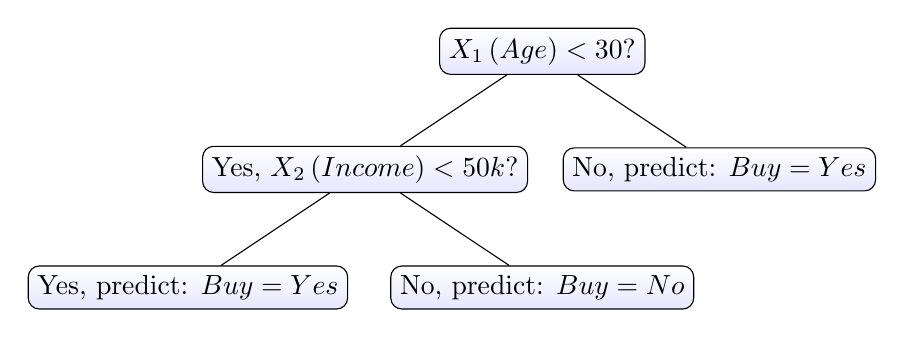
\begin{tikzpicture}[
            level 1/.style={sibling distance=45mm},
            level 2/.style={sibling distance=45mm},
            every node/.style={draw, rectangle, rounded corners, align=center, top color=white, bottom color=blue!10}
        ]

        \node {$X_1 \left(\text{Age}\right) < 30$?}
        child {
            node {Yes, $X_2 \left(\text{Income}\right) < 50\text{k}$?}
            child {
                node {Yes, predict: $\text{Buy} = \text{Yes}$}
            }
            child {
                node {No, predict: $\text{Buy} = \text{No}$}
            }
        }
        child {
            node {No, predict: $\text{Buy} = \text{Yes}$}
        };

        \end{tikzpicture}
    \end{center}

    This tree gives a \textbf{set of rules} for predicting whether a person buys a product, based on their age and income.
\end{examplebox}

\highspace
\begin{flushleft}
    \textcolor{Green3}{\faIcon{check-circle} \textbf{Why use Decision Tree?}}
\end{flushleft}
\begin{itemize}
    \item Easy to \textbf{visualize} and \textbf{explain}.
    \item Handle both \textbf{numerical} and \textbf{categorical} variables.
    \item Automatically detect \textbf{non-linear interactions}.
    \item Require \textbf{little data processing}.
    \item Form the base for powerful ensemble methods like Random Forest and Boosting.
\end{itemize}